\definecolor{mygrey}{rgb}{0.95, 0.95, 0.92}

\section{Bài 2}
Trong phần này chúng ta sẽ xem xét bài toán "Travelling salesman problem" (bài toán 
người giao hàng) - là một trong những bài toán kinh điển và nổi tiếng trong lớp các
bài toán về đồ thị nói chung và bài toán tìm đường đi ngắn nhất nói riêng. \\

\textit{Bài toán: Cho một danh sách các thành phố và khoảng cách từng cặp một, 
tìm đường đi ngắn nhất đi qua mỗi thành phố đúng một lần và quay về điểm xuất phát} \\


Chúng ta có thể mô hình bài toán trên bằng đồ thị như sau: \textit{Cho một đơn đồ thị đầy đủ, 
với các cạnh có trọng số, tìm đường đi xuất phát từ một đỉnh đi qua tất cả các đỉnh 
của đồ thị mỗi đỉnh đúng một lần với tổng trọng số (chi phí) nhỏ nhất.}

Trước hết chúng ta giải bài toán con đơn giản hơn là tìm đường đi với chi phí nhỏ nhất từ
một đỉnh $a$ tới đỉnh $z$ cho trước. Trong bài toán này, không nhất thiết ta phải đi qua 
tất cả các đỉnh của đồ thị. Có nhiều cách tiếp cận bài toán, cách đầu tiên mà ta có thể nghĩ 
ngay tới là \textit{vét cạn (brute force)}, tuy nhiên việc liệt kê toàn bộ cấu hình \
(toàn bộ các đường đi khả dĩ từ $a$ đến $z$) của bài toán rất tốn thời gian. Sau đây ta cùng
xem xét một thuật toán hiệu quả hơn là thuật toán Dijkstra.

\subsection{Thuật toán Dijkstra tìm đường đi ngắn nhất trên đồ thị}
Trước khi giải bài toán tổng quát, ta hãy xem xét một ví dụ đơn giản sau đây:

\begin{figure}[H] % places figure environment here   
    \centering % Centers Graphic
    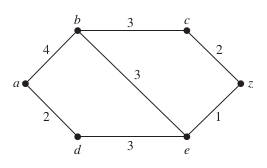
\includegraphics[width=0.4\textwidth]{assets/gr_01.png} 
    \caption{Ví dụ đơn đồ thị với trọng số } % Creates caption underneath graph
    \label{fig:gr_01}
\end{figure}

Tìm đường đi ngắn nhất từ đỉnh $a$ đến đỉnh $z$ trong đồ thị ở hình \ref{fig:gr_01}.\\ 

Trước hết, bắt đầu từ đỉnh $a$, có 2 đỉnh kết nối với $a$ là $b$ và $d$ với trọng số 
lần lượt là $4$ và $2$, đương nhiên $d$ là đỉnh gần $a$ nhất. Chúng ta có thể tìm đỉnh 
gần nhất thứ 2 bằng cách liệt kê tất cả các đường đi với $d$ là đỉnh bắt đầu và đỉnh 
kết thúc không nằm trong tập $\{a, d\}$. Tính từ đỉnh $d$, chỉ có một đường khả dĩ là $e$.
Từ đó ta có tập $\{a, d, e\}$. Tương tự như vậy ta tìm đỉnh tiếp theo với cạnh có trọng số 
nhỏ nhất với $e$ là đỉnh bắt đầu và đỉnh kết thúc không thuộc tập $\{a, d, e\}$, ta được 
đỉnh $z$. Đường đi cuối cùng là $a \to d \to e \to z$. \\

Ví dụ trên thể hiện nguyên lý tổng quát của thuật toán Dijkstra đó là đường đi từ đỉnh $a$
tói đỉnh $z$ có thể được xây dựng bằng cách liệt kê các đường đi và tìm đường có trọng số 
nhỏ nhất để thêm đỉnh đó vào tập đường đi.

Một cách tổng quát ta có thể trình bày thuật toán Dijkstra với lược đồ sau:

\begin{tcolorbox}[colframe=gray,colback=gray!20,left=10pt,right=10pt,top=10pt,bottom=10pt]
    \textbf{Thuật toán Dijkstra} \\
    $G$ là một đơn đồ thị kết nối với trọng số mỗi cạnh dương \\
    $G$ có các đỉnh $a = v_0, v_1, ..., v_n = z$, trọng số 
    $w(v_i, v_j)$ với $w(v_i, v_j) = \infty$ nếu $\{v_i, v_j\}$ không thuộc 
    tập cạnh của $G$

    \begin{itemize}
        \item [] for i = 1 to n 
        \begin{itemize}
            \item [] $L(v_i) = \infty$
        \end{itemize} 
        \item [] $L(a) = 0$
        \item [] $S = \emptyset $ (Khởi tạo các nhãn với nhãn của $a$ là $0$, 
        các nhãn khác bằng $\infty$ và tập $S$ rỗng)
        \item [] while $z \notin S$
        \begin{itemize}
          \item [] $u = a$ đỉnh không thuộc $S$ với $L(u)$ nhỏ nhất
          \item [] $S = S \cup \{u\}$
          \item [] for $v \notin S$
          \begin{itemize}
            \item [] if $L(u) + w(u,v) < L(v)$ then $L(v) = L(u) + w(u,v)$
            (Bước này thêm đỉnh gần nhất vào tập $S$ và cập nhật lại hàm chi phí)
          \end{itemize}
        \end{itemize}
        return $L(z)$ ($L(z)$ là độ dài của đường đi ngắn nhất từ $a$ tới $z$)
    \end{itemize}
  \end{tcolorbox}

\textit{Nhận xét: } Thuật toán Dijkstra đem lại
sự tường minh mà không phải quét qua toàn bộ cấu hình của bài toán, 
ta chỉ cập nhật đỉnh gần với đỉnh cuối cùng nhất, điều đó làm giảm không gian lưu 
trữ so với cách vét cạn (khi ta phải lưu toàn bộ đường đi và chi phí của mọi đường
đi khả dĩ từ đỉnh $a$ tới đỉnh $z$). Độ phức tạp của thuật toán là $O(n^2)$. 
Ta có thể dễ dàng thu được vì ban đầu khi chọn 1 đỉnh, ta cần $(n-1)$ phép so sánh
để tìm được đỉnh gần nhất đầu tiên, tiếp theo ta cần $(n-2)$ phép tính để tìm đỉnh 
gần nhất thứ 2, tiếp tục như vậy cho đến khi thu được đỉnh đích. Số phép tính là tổng 
từ $1$ đến $(n-1)$. \\

Trong thực tế lập trình, chúng ta không nhất thiết phải lưu giá trị cạnh bằng một 
số lớn (vô cùng) mà có thể đánh bằng $0$ và kiểm tra thêm một điều kiện trong vòng 
lặp để tránh sự cồng kềnh của ma trận kề. \\

\href{https://github.com/batman0911/dma_homework/blob/master/hw_02/src/shortest_path.ipynb}{python code} 
    cho bài toán.


\subsection{Bài toán người đưa hàng (TSP)}
Trong mục này chúng ta sẽ xem xét bài toán người đưa hàng đã đề cập ở đầu bài.
Sau khi giải bài toán tìm đường đi ngắn nhất ở mục trước, ta biết rằng bài toán
người đưa hàng không gì khác ngoài việc tìm được đi ngắn nhất khi ta đặt điểm
kết thúc chính là điểm bắt đầu. 
\subsubsection{Thuật toán tìm nghiệm chính xác}
Độ phức tạp thuật toán vét cạn và là $O (n!)$.
Độ phức tạp này tăng rất nhanh theo $n$ . Ví dụ khi bắt đầu từ 1 đỉnh, ta có $(n-1)!$
chu trình Hamilton, tới đỉnh thứ 2 ta còn $(n-2)!$ chu trình Hamilton và tiếp tục như vậy.
Bởi vì ta có thể đi theo thứ tự ngược lại trong chu trình Hamilton nên số chu trình cần
sinh ra để có được lời giải là $(n-1)!/2$. Với số đỉnh bằng $25$, số chu trình được sinh 
ra là $24!/2 \sim 3.1 \times 10^{23}$ - một con số lớn khủng khiếp. Trong thực tế, 
một đơn vị vận chuyển như \textit{Giao hàng tiết kiệm} giao hàng triệu đơn hàng mỗi ngày 
tới các địa điểm khác nhau! Do đó ta gần như không thế tìm được lời giải chính xác của bài 
toán TSP trong thực tế mà cần phải sử dụng các phương pháp xấp xỉ để tìm được một 
đường đi \textit{đủ tốt}.

\subsubsection{Phương pháp xấp xỉ}
Chúng ta sẽ cố gắng đi tìm một cấu hình (chu trình Hamilton) với chi phí không vượt quá
một \textit{ngưỡng} nhất định. Hay nói cách khác $L(H^*_{G}) \leq L(H_{G}) \leq cL(H^*_{G})$,
trong đó $L(H_G)$ là hàm chi phí (tổng các trọng số) của một chu trình Hamilton với
đồ thị $G$ và $H^*_G$ là cấu hình tối ưu của bài toán. Có những thuật toán tìm nghiệm 
xấp xỉ với thời gian đa thức trên đồ thị thỏa mãn bất đẳng thức tam giác với $c = 3/2$. \\

Sử dụng ý tưởng của thuật toán Dijkstra, ta thêm vào tập đỉnh đã đi qua đỉnh lân cận 
gần nhất cho đến khi toàn bộ tập đỉnh đã được đi qua. Độ phức tạp của thuật toán là $O(n^2)$
và ta sẽ cùng xem hệ số $c$ với thuật toán này bằng bao nhiêu. \\

Trước hết, đồ thị $G$ phải thỏa mãn điều kiện bất đẳng thức tam giác 
$w_{ik} + w_{kj} \geq w_{ij}$, với $w_{st}$ là trọng số của cạnh nối đỉnh $s$ và đỉnh $t$.
Điều này cũng khá thực tế khi chi phí bay thẳng từ Hà Nội đến Sài Gòn nên nhỏ hơn là phải 
bay từ Hà Nội vào Đà Nẵng rồi từ Đà Nẵng đi Sài Gòn!

\href{https://github.com/batman0911/dma_homework/blob/master/hw_02/src/travelling_salesman.ipynb}{python code} 
    cho bài toán. \\